%!TEX TS-program = pdflatex
%!TEX root = tesi.tex
%!TEX encoding = UTF-8 Unicode

\chapter{Il Problema}
All'inizio di questo capitolo verranno illustrati forma e fine ultimo dei pezzi meccanici analizzati.
Seguirà una descrizione sommaria del processo industriale e delle macchine che manipolano e depositano la colla all'interno dei pezzi, nonché del sistema di acquisizione immagini.
Si conclude con una formalizzazione del problema da risolvere e le metriche con cui valutare la soluzione proposta.

\section{Le carcasse per motori elettrici}

Osservando le fotografie in figura~\ref{fig:carc}, possono essere definite le caratteristiche principali delle carcasse:
\begin{itemize}
  \item il pezzo ha una struttura cilindrica cava;
  \item il fondo presenta tre gradini;
  \item sono presenti due balze (nella foto laterale se ne vede soltanto una), posizionate una di fronte all'altra, prima del primo gradino;
  \item i supporti alla bocca della carcassa presentano due fori.
\end{itemize}
Il pezzo è stato pensato per avvolgere e proteggere motori elettrici.
Nello specifico i pezzi in foto, sui quali è stato svolto lo studio, sono carcasse per motori elettrici per tergicristalli.
I due fori aiuteranno a fissare con delle viti il pezzo su dei supporti in plastica.
All'interno della cavità verrà depositata della colla liquida, successivamente verrà alloggiato il motore.
La colla verrà fatta solidificare tramite calore, in modo che il motore, una volta posizionato, non possa vibrare all'interno della carcassa, evitando che eventuali urti possano danneggiarlo.
Dalle foto in figura~\ref{fig:carc} si può notare che la colla è distribuita in modo da formare un anello ad una altezza di circa $4cm$ dal fondo della carcassa.

La colla è stata depositata correttamente se:
\begin{enumerate}
  \item l'anello non presenta né sbavature né discontinuità;
  \item sul fondo non c'è presenza di colla.
\end{enumerate}
In questo documento ci concentreremo esclusivamente sul secondo punto, infatti la presenza di colla sul fondo della carcassa causa il malfunzionamento del motorino dopo un limitato tempo d'utilizzo, molto inferiore al tempo di vita atteso.
Per questo motivo è fondamentale che la colla venga depositata correttamente.

\begin{figure}[h]
  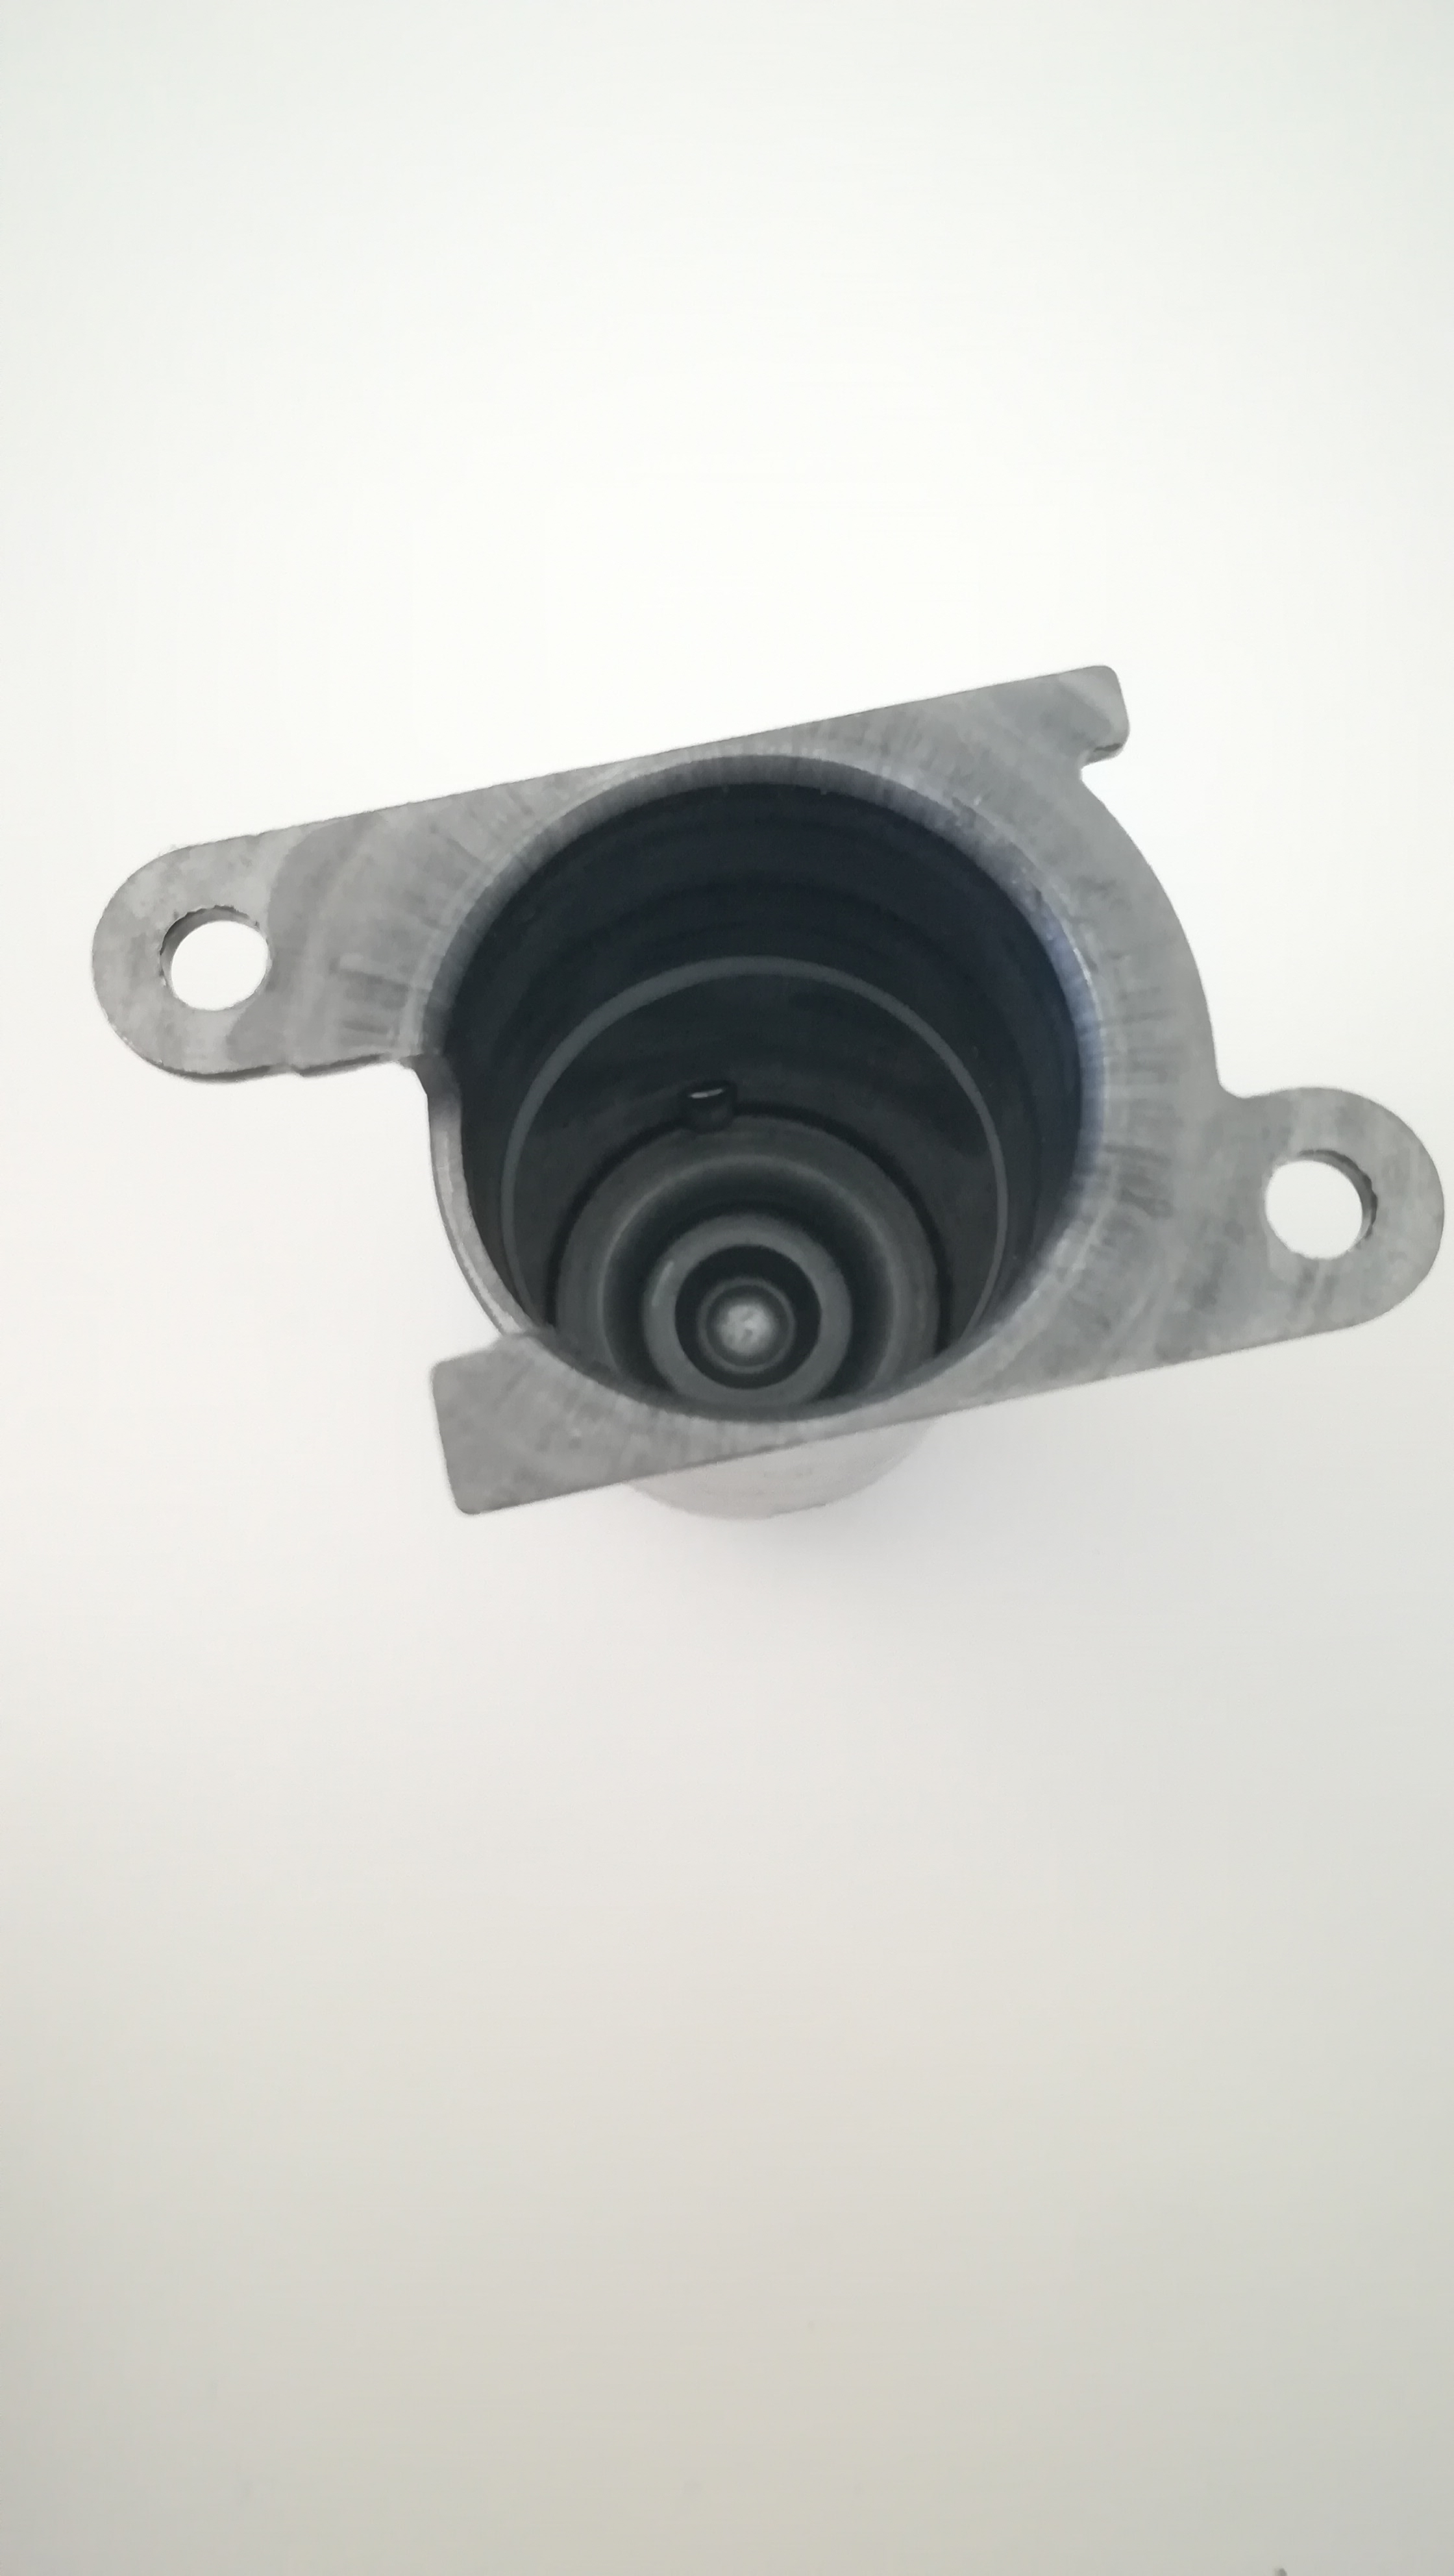
\includegraphics[width=0.49\textwidth]{carcassa_da_sopra}
  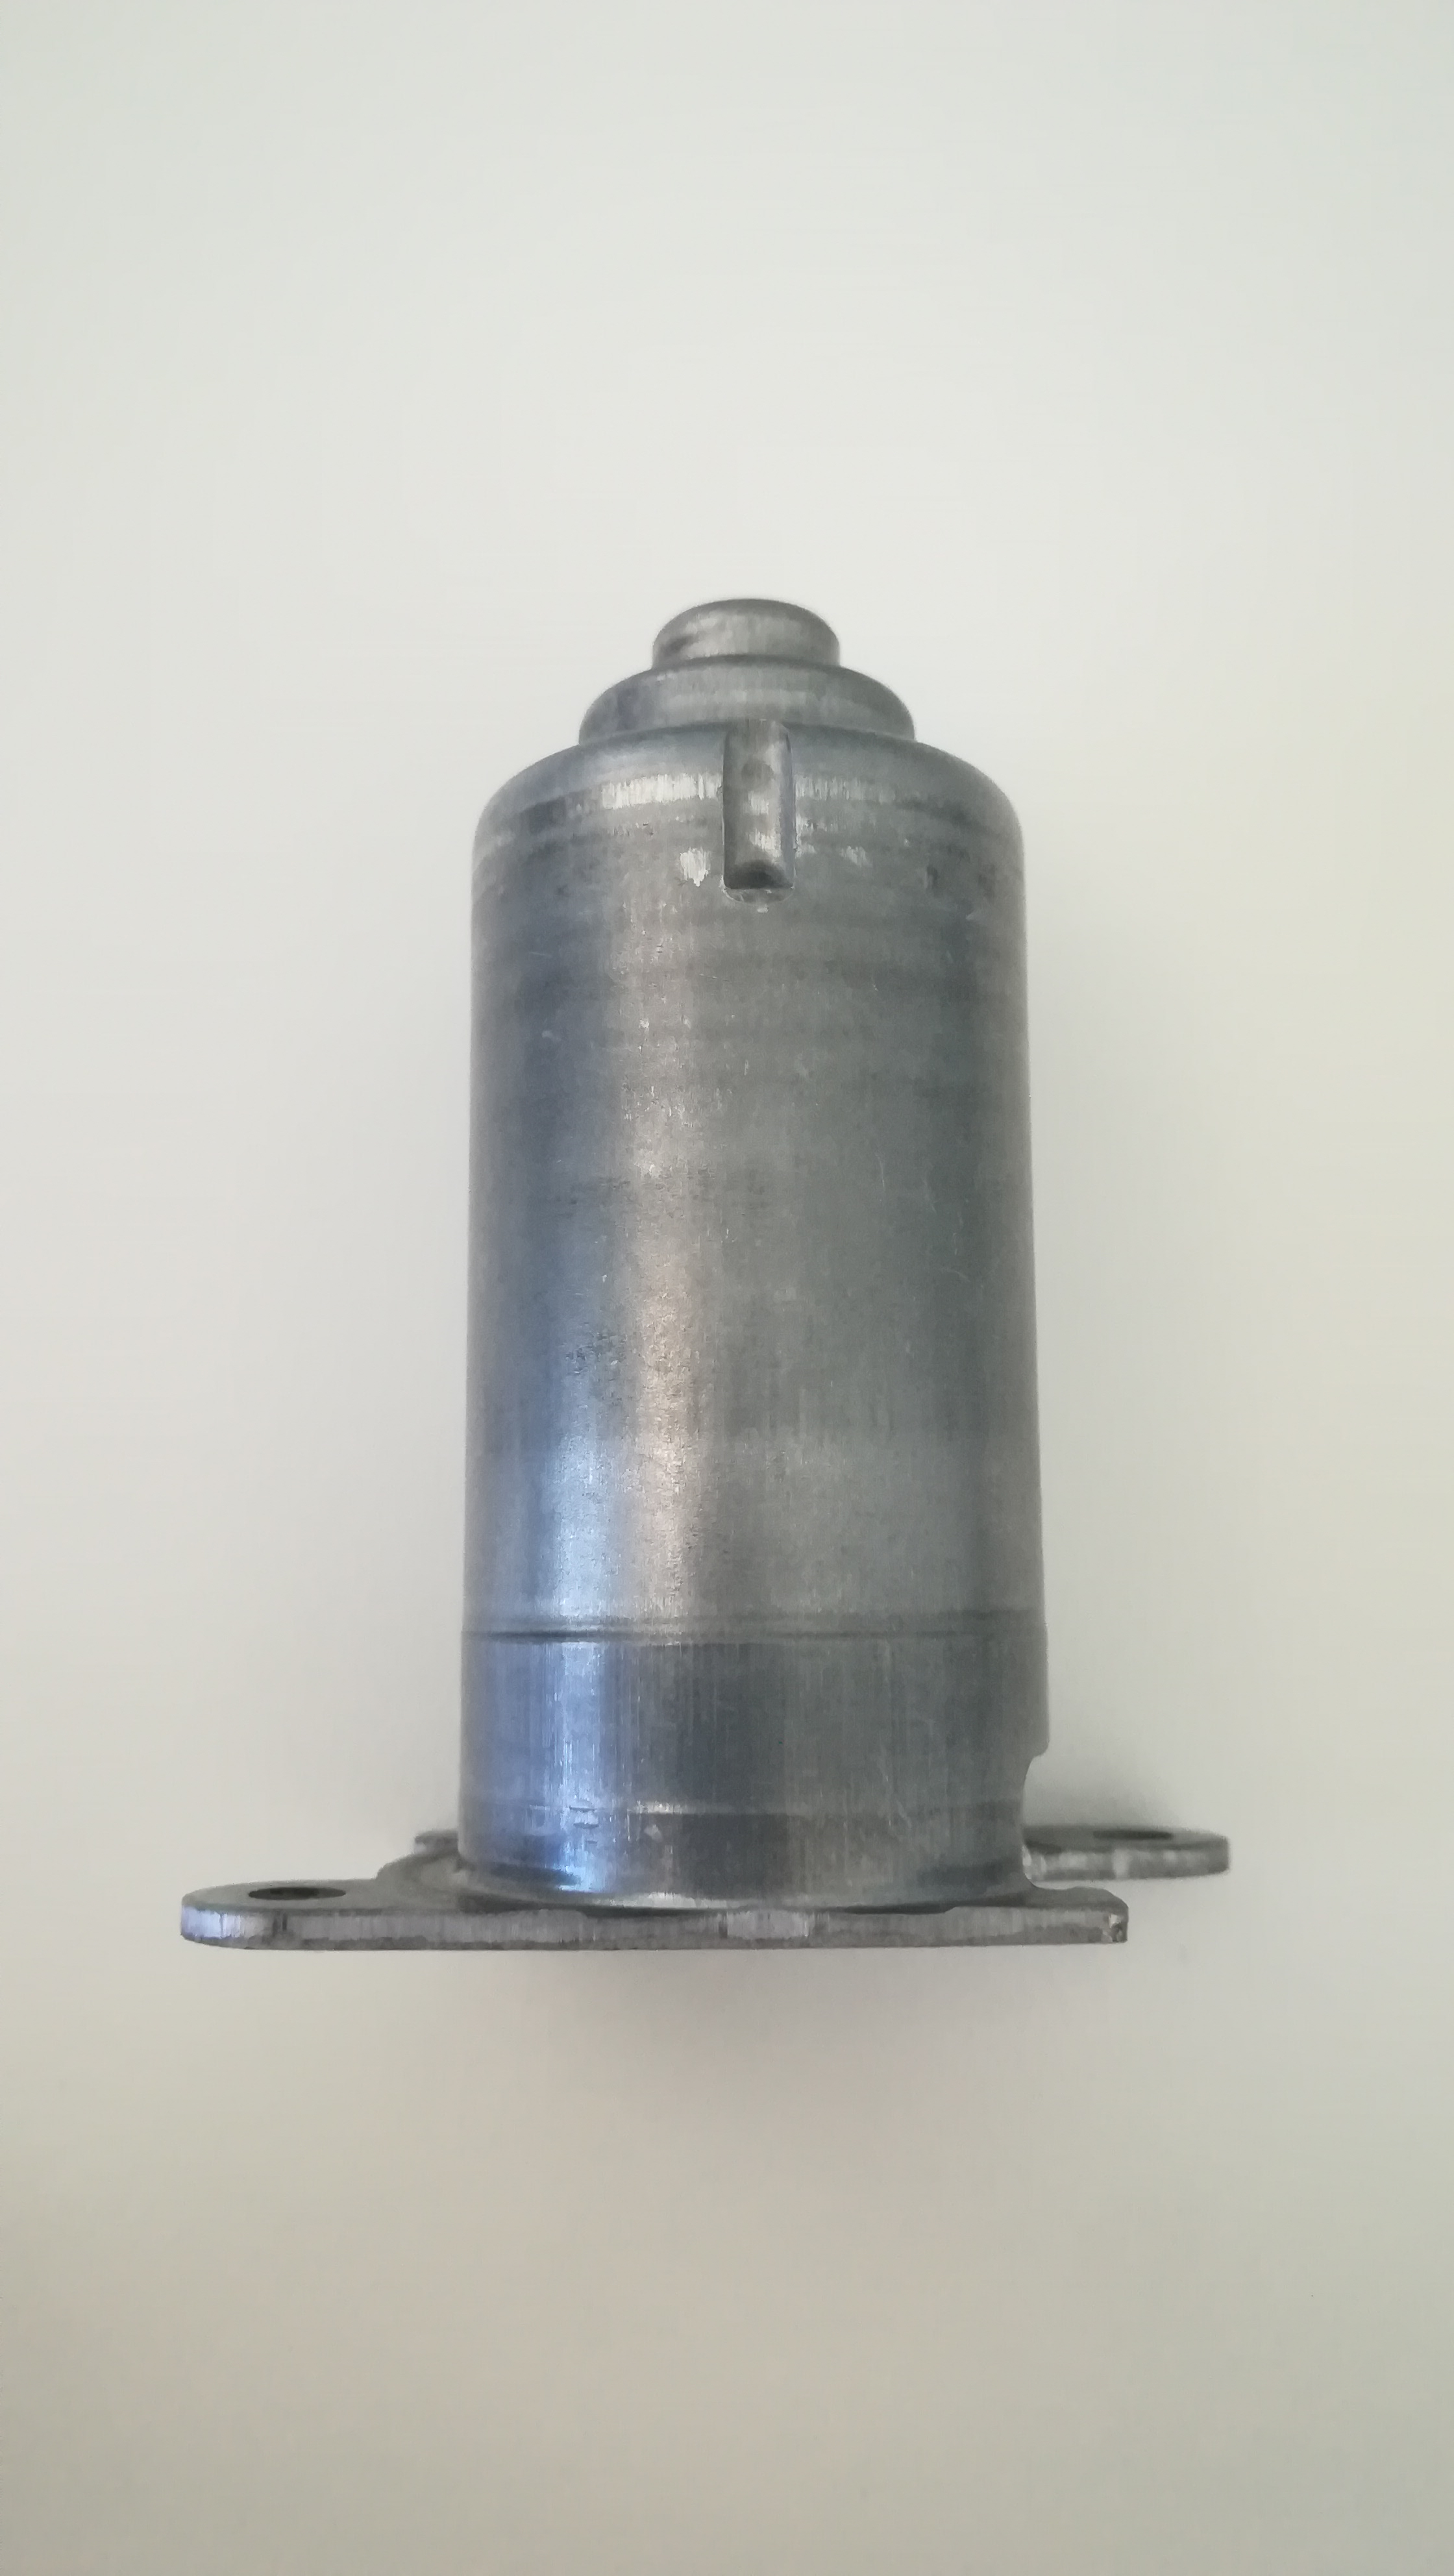
\includegraphics[width=0.49\textwidth]{carcassa_di_lato}
  \caption{Visioni laterale e superiore di una carcassa}
  \label{fig:carc}
\end{figure}

\clearpage

\section{Il processo di produzione}
Chiarire le modalità con cui le carcasse vengono manipolate, la colla viene depositata e le foto vengono acquisite risulta fondamentale.
Senza queste informazioni mancherebbe la base sulla quale costruire ipotesi e considerazioni riguardo le immagini del \textit{dataset}.
Analizzando le condizioni in cui le foto vengono scattate, si definiscono i vincoli ed i confini entro i quali le soluzioni proposte possono considerarsi verosimili ed applicabili al mondo reale.

Le carcasse, già presenti in grandi quantità in magazzino, raggiungono il macchinario e vengono caricate, con la concavità rivolta verso l'alto, su un disco rotante.
%TODO termini giusti sotto?
%TODO il processo è giusto?
Ad ogni ciclo macchina la colla, tramite due ugelli, viene depositata simultaneamente su due carcasse distinte.
Al contempo due sonde dotate di luce scendono nelle due carcasse su cui la colla era stata depositata il ciclo precedente, fino ad una distanza di circa $3cm$ dal fondo.
Le carcasse ritenute conformi procedono lungo un rullo trasportatore, mentre quelle che non sono idonee vengono scartate.

Vanno precisati vari aspetti.
Le carcasse, nonostante siano tutte dello stesso tipo, possono differire per quanto riguarda colore, graffi superficiali, sporco, incrostazioni oppure macchie.
Inoltre non vengono orientate tutte allo stesso modo rispetto all'asse verticale: questo ha delle ripercussioni dirette sulle foto raccolte, infatti le due balze non si presenteranno in posizioni fisse.

Il sistema assicura che le foto vengano scattate sempre alla stessa profondità e che la sonda sia centrata rispetto al pezzo (considerando come centro il centro della cavità cilindrica).
La distanza fissa è condizione sufficiente per garantire la messa a fuoco di ognuno dei tre gradini sul fondo.
Purtroppo non sono stati specificati dei vincoli riguardo l'illuminazione.

Si fa notare che il processo appena descritto viene eseguito da almeno due macchinari distinti, ovviamente questo aggiunge un ulteriore grado di sfida: non si può supporre che i macchinari siano sempre calibrati esattamente allo stesso modo.
%La nostra soluzione dovrà quindi essere in grado di resistere a TODO completare commento

In conclusione le foto che saranno da analizzare vengono raccolte da un totale di quattro fotocamere distinte, delle quali si assicura
\begin{itemize}
  \item con un grado di precisione soddisfacente la distanza dal fondo;
  \item con un grado di precisione accettabile la centratura delle immagini.
\end{itemize}
%TODO riassumere anche le caratteristiche delle carcasse?

\todo[inline]{qua riprendo i dati sulle percentuali di errore ?}
